\documentclass{article}

\usepackage{amsmath,amssymb,amsthm,mathtools,mathrsfs}
\usepackage[margin=1in]{geometry}
\usepackage{tikz}

\usetikzlibrary{arrows,automata}

\newtheorem{thm}{Theorem}
\newtheorem{lem}{Lemma}
\newtheorem{defin}{Definition}
\newtheorem*{cor}{Corollary}

\newenvironment{subproof}{%
  \begin{proof}[Subproof]%
}{%
  \end{proof}%
}

\begin{document}

First let us lay out some definitions.
These should probably be pretty familiar but we want to be extra explicit.

\begin{defin}
We shall define $\mathbb{A}$ to be a infinitely large set.
We will call its members \textbf{Atoms}.
\end{defin}

\begin{defin}
We shall define $\mathbb{V}$ to be a infinitely large set disjoint from the set of atoms.
We will call its members \textbf{Free Variables}.
\end{defin}

We won't talk about the internal structure of atoms and free variables, we only insist that the two are disjoint.
Now in practice there are no limitations on the number of atoms and free variables available but for convenience we will take atoms to be any capital Latin letter and free variables to be any lower case Greek letter.

\begin{defin}
A \textbf{well formed formula} (in the \L ukasievicz system) will be defined as follows:
\begin{enumerate}
\item Every atom is a well formed formula.
\item If $\Phi$ is a well formed formula $\neg\Phi$ is also a well formed formula.
\item If both $\Phi$ and $\Psi$ are well formed formulae then $(\Phi\rightarrow\Psi)$ is a well formed formula.
\item No other statements are well formed formulae.
\end{enumerate}
We will call the set of all well formed formulae $\mathcal{W}$.
\end{defin}


\begin{defin}
A \textbf{formula} (in the \L ukasievicz system) will be defined as follows:
\begin{enumerate}
\item Every atom is a formula.
\item Every free variable is a formula.
\item If $\Phi$ is a formula $\neg\Phi$ is also a formula.
\item If both $\Phi$ and $\Psi$ are formulae then $(\Phi\rightarrow\Psi)$ is a formula.
\item No other statements are formulae.
\end{enumerate}
We will call the set of all formulae $\mathcal{F}$.
\end{defin}

When talking about arbitrary formulae we will use capital Greek letters to stand in for complex statments.
For example if we wanted to talk about statements with $\rightarrow$ at the top level we would use the notation $\Phi \rightarrow \Psi$.
This is usually what free variables are used for but because free variables are objects we are concerned with we need to operate at the meta level.
This is purely notational.

\begin{defin}
Two formulae are \textbf{equal} if they are both generated by the same path in the grammar.
\begin{align*}
(\Phi \rightarrow \Psi) = (\Omega \rightarrow \Sigma) &\iff (\Phi = \Omega) \land (\Psi = \Sigma) \\
\neg \Phi = \neg \Psi &\iff \Phi = \Psi
\end{align*}
Formulae comprised solely of an atom or variable inherit equality from the atom or variable they are comprised of.
\end{defin}

\begin{defin}
The \textbf{set of free variables appearing in} a formula $\Phi$ will be denoted as $\Phi^\mathbb{V}$.
\setlength{\tabcolsep}{1pt}
\begin{center}
	\begin{tabular}{rclc}
		                               & $(\Phi \rightarrow \Psi)^\mathbb{V}$ & $=$ & $ \Phi^\mathbb{V} \cup \Psi^\mathbb{V}$ \\
		                               & $(\neg \Phi)^\mathbb{V}            $ & $=$ & $ \Phi^\mathbb{V}               $ \\
		$\Phi \in \mathbb{A} \implies$ & $\Phi^\mathbb{V}                   $ & $=$ & $ \{\}                    $ \\
		$\Phi \in \mathbb{V} \implies$ & $\Phi^\mathbb{V}                   $ & $=$ & $ \{\Phi\}                $
	\end{tabular}
\end{center}
\end{defin}

\begin{defin}
The \textbf{set of atoms appearing in} a formula $\Phi$ will be denoted as $\Phi^\mathbb{A}$.
\setlength{\tabcolsep}{1pt}
\begin{center}
	\begin{tabular}{rclc}
		                               & $(\Phi \rightarrow \Psi)^\mathbb{A}$ & $=$ & $ \Phi^\mathbb{A} \cup \Psi^\mathbb{A}$ \\
		                               & $(\neg \Phi)^\mathbb{A}            $ & $=$ & $ \Phi^\mathbb{A}               $ \\
		$\Phi \in \mathbb{V} \implies$ & $\Phi^\mathbb{A}                   $ & $=$ & $ \{\}                    $ \\
		$\Phi \in \mathbb{A} \implies$ & $\Phi^\mathbb{A}                   $ & $=$ & $ \{\Phi\}                $
	\end{tabular}
\end{center}
\end{defin}
\begin{defin}
The function $f : A \mapsto B$ \textbf{constrained to} a set $C \subseteq A$, denoted $f \mid A$ is a new function mapping
members of $C$ to members of $B$ such that:

\begin{align*}
\forall x \in C : (f \mid C) (x) = f (x)
\end{align*}
\end{defin}

\begin{defin}
If we have a formula $\Phi$ and a function $f$, which maps free variables to formulae,
the \textbf{assignment} of $\Phi$ by $f$, denoted $\Phi \lhd f$, will be defined as such:
\begin{align*}
(\Phi \rightarrow \Psi) \lhd f &= (\Phi \lhd f \rightarrow \Psi \lhd f) \\
(\neg \Phi) \lhd f &= \neg (\Phi \lhd f) \\
\Phi \in \mathbb{A} \implies \Phi \lhd f &= \Phi \\
\Phi \in \mathbb{V} \implies \Phi \lhd f &= f(\Phi) \\
\end{align*}
\end{defin}

One can think of assignment as applying a function $f$ to every free variable in the formula.
In this way it ``\textit{assigns}" each free variable.

\begin{lem}
If $\Phi \lhd f = \Phi \lhd g$ then $f \mid \Phi^\mathbb{V} = g \mid \Phi^\mathbb{V}$.
\end{lem}
\begin{proof}
We will prove this via structural induction.

First we will consider the case where $\Phi$ is an atom.
By definiton $\Phi^\mathbb{V} = \{\}$.
For any two functions $f$ and $g$, $f \mid \{\} = g \mid \{\}$,
thus the claim is true.

Now we consider the case where $\Phi$ is a free variable.
By definiton $\Phi^\mathbb{V} = \{\Phi\}$.
Thus the domain of our functions $f\mid\Phi^\mathbb{V}$ and $g\mid\Phi^\mathbb{V}$ is $\{\Phi\}$.
Since $\Phi \lhd f = \Phi \lhd g$, by the definition of assignment
\begin{align*}
f(\Phi) &= g(\Phi) \\
(f\mid\Phi^\mathbb{V})(\Phi) &= (g\mid\Phi^\mathbb{V})(\Phi)
\end{align*}
Since we have confirmed that the two functions are the same across their entire domains they must be equal.

Now let us consider the case where $\Phi = \neg \Psi$ and where we know that
\begin{align*}
\forall f,g: \Psi \lhd f = \Psi \lhd g \implies f\mid\Phi^\mathbb{V}=g\mid\Psi^\mathbb{V}
\end{align*}
If we have two arbitrary functions $f$ and $g$ where $\Phi\lhd f=\Phi\lhd g$.
\begin{align*}
\Phi\lhd f        &= \Phi\lhd g      \\
(\neg\Psi)\lhd f &= (\neg\Psi)\lhd g \\
\neg(\Psi\lhd f) &= \neg(\Psi\lhd g) \\
\Psi\lhd f &= \Psi\lhd g             \\
f\mid\Psi^\mathbb{V} &= g\mid\Psi^\mathbb{V}
\end{align*}
By definition $\Phi^\mathbb{V} = (\neg\Psi)^\mathbb{V} = \Psi^\mathbb{V}$ thus
\begin{align*}
f\mid\Phi^\mathbb{V} &= g\mid\Phi^\mathbb{V}
\end{align*}

Lastly let us consider that $\Phi = (\Psi\rightarrow\Omega)$, and that
\begin{align*}
\forall f,g: & \: \Psi   \lhd f = \Psi   \lhd g \implies f\mid\Phi^\mathbb{V}  =g\mid\Psi^\mathbb{V}   \\
\forall f,g: & \: \Omega \lhd f = \Omega \lhd g \implies f\mid\Omega^\mathbb{V}=g\mid\Omega^\mathbb{V}
\end{align*}
Let's consider two functions $f$ and $g$ such that $\Phi\lhd f=\Phi\lhd g$.
\begin{align*}
\Phi\lhd f                          &= \Phi\lhd g                              \\
(\Psi\rightarrow\Omega)\lhd f       &= (\Psi\rightarrow\Omega)\lhd g           \\
(\Psi\lhd f\rightarrow\Omega\lhd f) &= (\Psi\lhd g\rightarrow\Omega\lhd g)     \\
\Psi\lhd f = \Psi\lhd g             &\land \Omega\lhd f = \Omega\lhd g         \\
f\mid\Psi^\mathbb{V} = g\mid\Psi^\mathbb{V}     &\land f\mid\Omega^\mathbb{V} = g\mid\Omega^\mathbb{V} \\
\end{align*}

\end{proof}

\begin{lem}
\begin{align*}
(\Delta\lhd l)^\mathbb{V}
= \bigcup_{\delta \in \Delta} (l(\delta))^\mathbb{V}
\end{align*}
\end{lem}
\begin{proof}
Let us consider a statment $\Delta$ assigned by a function $l$.
If $\Delta$ is of the form $(\Delta_1\rightarrow\Delta_2)$ then
\begin{align*}
((\Delta_1\rightarrow\Delta_2)\lhd l)^\mathbb{V}
&= ((\Delta_1\lhd l)\rightarrow(\Delta_2\lhd l))^\mathbb{V} \tag{Definition of Assignment} \\
&= (\Delta_1\lhd l)^\mathbb{V}\cup(\Delta_2\lhd l)^\mathbb{V} \tag{Definition of Free Variable Set}
\end{align*}
If $\Delta$ is of the form $\neg \Delta_0$ then
\begin{align*}
((\neg \Delta_0)\lhd l)^\mathbb{V}
&= (\neg (\Delta_0\lhd l))^\mathbb{V} \tag{Definition of Assignment} \\
&= (\Delta_0\lhd l)^\mathbb{V} \tag{Definition of Free Variable Set} \\
\end{align*}
If $\Delta$ is an atom
\begin{align*}
(\Delta_0\lhd l)^\mathbb{V}
&= \Delta_0^\mathbb{V} \tag{Definition of Assignment} \\
&= \{\} \tag{Definition of Free Variable Set} \\
\end{align*}
If $\Delta$ is a free variable
\begin{align*}
(\Delta_0\lhd l)^\mathbb{V}
&= (l(\Delta_0))^\mathbb{V} \tag{Definition of Assignment} \\
&= \{l(\Delta_0)\} \tag{Definition of Free Variable Set} \\
\end{align*}
Thus, by induction it is the case that 
\begin{align*}
(\Delta\lhd l)^\mathbb{V}
= \bigcup_{\delta \in \Delta^\mathbb{V}} (l(\delta))^\mathbb{V}
\end{align*}
\end{proof}

\begin{defin}
The \textbf{chain} of two assignment functions, $f$ and $g$, denoted $g \diamond f$ is defined as follows:
\begin{align*}
(f \diamond g) (x) = (f (x)) \lhd g
\end{align*}
alternatively via partial application we could write this as
\begin{align*}
(f \diamond g) = ((\lhd g)\circ f)
\end{align*}
\end{defin}

\begin{lem}
\begin{align*}
(\Phi \lhd f) \lhd g = \Phi \lhd (f \diamond g)
\end{align*}
\end{lem}
\begin{proof}
Here we will use a pretty straightforward proof by induction.
If we assume that $\Phi$ is of the form $(\Phi_1 \rightarrow \Phi_2)$ and
\begin{gather*}
(\Phi_1 \lhd f) \lhd g = \Phi_1 \lhd (f \diamond g) \\
\land \\
(\Phi_2 \lhd f) \lhd g = \Phi_2 \lhd (f \diamond g)
\end{gather*}
We can show
\begin{align*}
((\Phi_1 \rightarrow \Phi_2) \lhd f) \lhd g &= (\Phi_1 \lhd f \rightarrow \Phi_2 \lhd f) \lhd g                     \tag{Definition of Assignment}\\
                                            &= ((\Phi_1 \lhd f) \lhd g \rightarrow (\Phi_2 \lhd f) \lhd g)          \tag{Definition of Assignment}\\
                                            &= (\Phi_1 \lhd (f \diamond g) \rightarrow (\Phi_2 \lhd f) \lhd g)      \tag{Inductive Hypothesis I}\\
                                            &= (\Phi_1 \lhd (f \diamond g) \rightarrow \Phi_2 \lhd (f \diamond g))  \tag{Inductive Hypothesis II}\\
                                            &= (\Phi_1 \rightarrow \Phi_2) \lhd (f \diamond g)                      \tag{Definition of Assignment}\\
\end{align*}
If we assume that $\Phi$ is of the form $\neg\Phi$ and $(\Phi \lhd f) \lhd g = \Phi \lhd (f \diamond g)$ we can show
\begin{align*}
((\neg \Phi) \lhd f) \lhd g &= (\neg (\Phi \lhd f)) \lhd g     \tag{Definition of Assignment} \\
                            &= \neg ((\Phi \lhd f) \lhd g)     \tag{Definition of Assignment} \\
                            &= \neg (\Phi \lhd (f \diamond g)) \tag{Inductive Hypothesis}     \\
                            &= (\neg \Phi) \lhd (f \diamond g) \tag{Definition of Assignment} \\
\end{align*}
If we assume that $\Phi \in \mathbb{A}$ we can show that
\begin{align*}
(\Phi \lhd f) \lhd g &= \Phi \lhd g              \tag{Definition of Assignment} \\
                     &= \Phi                     \tag{Definition of Assignment} \\
                     &= \Phi \lhd (f \diamond g) \tag{Definition of Assignment} \\
\end{align*}
If we assume that $\Phi \in \mathbb{V}$ we can show that
\begin{align*}
(\Phi \lhd f) \lhd g &= f(\Phi) \lhd g           \tag{Definition of Assignment} \\
                     &= (f \diamond g) (\Phi)    \tag{Definition of Assignment} \\
                     &= \Phi \lhd (f \diamond g) \tag{Definition of Chain} \\
\end{align*}
Thus via induction we know that $(\Phi\lhd f)\lhd g=\Phi\lhd(f\diamond g)$.
\end{proof}

This lemma means we can treat chaining as function composition for assignment.

\begin{defin}
Let a formula $\Phi$ be a \textbf{subformula} of a formula $\Psi$
if and only if there exists some function $f$ such that the assignment of $\Psi$ by $f$ is equal to $\Phi$.
We will use the usual $\subseteq$ symbol to denote subformula.

\begin{align*}
\Phi \subseteq \Psi \iff \exists f: \Psi \lhd f = \Phi
\end{align*}
\end{defin}

\begin{defin}
Let the \textbf{intersection} (denoted $\cap$) of two formulae $\Phi$ and $\Psi$ be
the set of all well formed formulae $\Omega$ such that there is an assignment that makes $\Omega$ equal to both $\Phi$ and $\Psi$.

\begin{align*}
\Phi \cap \Psi = \left\{\Omega \in \mathcal{W} \mid \exists f: (\Phi \lhd f = \Omega \land \Psi \lhd f = \Omega)\right\}
\end{align*}
\end{defin}

Note that the intersection of $\Phi$ and $\Psi$ is \textit{not}

\begin{align*}
\left\{\Omega \in \mathcal{W} \mid \Omega \subseteq \Phi \land \Omega \subseteq \Psi\right\}
\end{align*}

the assignment that makes $\Omega$ equal $\Phi$ and the assignment that makes $\Omega$ equal $\Psi$ must be the same.

As a counter example

\begin{align*}
\phi \cap (\phi \rightarrow \phi) = \{\}
\end{align*}

despite the fact $(A \rightarrow A)$ is a member of both formulae.

\begin{defin}
A set of well formed formulae is \textbf{equivalent} to a formula if every member of the set is a subformula of the formula and
every well formed subformula of the formula is a member of the set.
\begin{align*}
A \equiv \Phi \iff \forall \Omega \in \mathcal{F}: \Omega \in A \iff (\Omega \subseteq \Phi \land \Omega \in \mathcal{W})
\end{align*}
\end{defin}

\begin{lem}
If $\Phi \cap \Psi \equiv \Omega$ then $\exists f: \Phi \lhd f = \Omega \land \Psi \lhd f = \Omega$
\end{lem}
\begin{proof}
Let us have $\Phi$ and $\Psi$ such that $\Phi \cap \Psi \equiv \Omega$.
Now let us consider a function $f$ that is a bijection between the set of free variables and the set of atoms that do not appear in $\Omega$.
\begin{equation*}
f : \mathbb{V} \mapsto \mathbb{A}\setminus\Omega^{\mathbb{A}}
\end{equation*}
Let us call the application of $f$ on $\Omega$, $\Xi$.
Via the definiton of equivalence, $\Xi$ must be a member of the intersecton.
Now since $\Xi$ is a member of the intersection, by definition, there is some $h$ such that
\begin{align*}
\Phi \lhd h = \Xi \land \Psi \lhd h = \Xi
\end{align*}
Now let us consider a function $g$, from formulae to formulae, defined as follows:
\begin{gather*}
g (\neg\Phi) = \neg (g \Phi) \\
g (\Phi_1 \rightarrow \Phi_2) = (g(\Phi_1)\rightarrow g(\Phi_2)) \\
\Phi \in \Omega^{\mathbb{V}} \implies g(\Phi) = \Phi\\
\Phi \in \mathbb{A}\setminus \Omega^{\mathbb{V}} \implies g(\Phi) = f^{-1} (\Phi)\\
\end{gather*}
This function replaces all atoms not in $\Omega$ with the free variables that map to them under $f$.
We will now show that $g (\Xi) = g (\Omega \lhd f) = \Omega$.
If we consider that $\Omega$ is of the form $\neg \Omega_0$ we see that:
\begin{align*}
   g ((\neg \Omega_0) \lhd f)
&= g (\neg (\Omega_0 \lhd f)) \tag{Definition of Assignment}\\
&= \neg(g (\Omega_0 \lhd f))  \tag{Definition of $g$}       
\end{align*}
If $\Omega$ is of the form $(\Omega_1 \rightarrow \Omega_2)$ we see that:
\begin{align*}
   g ((\Omega_1 \rightarrow \Omega_2) \lhd f)
&= g ((\Omega_1 \lhd f) \rightarrow (\Omega_2 \lhd f))      \tag{Definition of Assignment} \\
&=((g (\Omega_1 \lhd f)) \rightarrow (g (\Omega_2 \lhd f))) \tag{Definition of $g$}
\end{align*}
If $\Omega$ is an atom, it must be the case that $\Omega^\mathbb{A} =\{\Omega\}$, thus
\begin{align*}
   g (\Omega \lhd f)
&= g (\Omega) \tag{Definition of Assignment} \\
&= \Omega     \tag{Definition of $g$}
\end{align*}
If $\Omega$ is a free variable then $f (\Omega)$ must be an atom not in $\Omega^\mathbb{A}$.
Thus
\begin{align*}
   g (\Omega \lhd f)
&= g (f (\Omega)) \tag{Definition of Assignment} \\
&= f^{-1} (f (\Omega)) \tag{Definition of $g$} \\
&= \Omega
\end{align*}
Thus by structural induction $g(\Xi) = \Omega$.

Now by this fact we will show the function $g \circ h$ assigns $\Phi$ to $\Omega$.
\begin{equation*}
\Phi \lhd (g \circ h) = \Omega
\end{equation*}
In order to do this we wish to prove that
\begin{equation*}
\Phi \lhd (g \circ h) = g (\Phi \lhd h)
\end{equation*}
First we will show that $\Phi^\mathbb{A} \subseteq \Omega^\mathbb{A}$.
Let us assume that there is some atom in $\Phi^\mathbb{A}$ that is not in $\Omega^\mathbb{A}$, we will call this atom $A$.
We will define a function $j : \mathbb{V} \mapsto \mathbb{A} \setminus \{A\}$.
$A$ must not be in $(\Omega \lhd j)^\mathbb{A}$, and $\Omega \lhd j$ must be a well formed formula.
However, $\Omega \lhd j$ must be an assignment of $\Phi$, and every assignment of $\Phi$ must contain $A$, thus $\Omega \lhd j$ must contain $A$.
This is a contradiction thus our premise was false.
There is no atom that appears in $\Phi$ that does not appear in $\Omega$.

We will now prove the remainer by induction.

If $\Phi$ is of the form $(\Phi_1 \rightarrow \Phi_2)$ then
\begin{align*}
   \Phi \lhd (g \circ h)
&= (\Phi_1 \rightarrow \Phi_2) \lhd (g \circ h)                 \\
&= (\Phi_1 \lhd (g \circ h) \rightarrow \Phi_2 \lhd (g \circ h)) \tag{Definition of Assignment} \\
&= (g(\Phi_1 \lhd h) \rightarrow \Phi_2 \lhd (g \circ h))       \tag{Inductive Hypothesis I} \\
&= (g (\Phi_1 \lhd h) \rightarrow g(\Phi_2 \lhd h))            \tag{Inductive Hypothesis II} \\
&= g((\Phi_1 \lhd h) \rightarrow (\Phi_2 \lhd h))              \tag{Definition of $g$} \\
&= g((\Phi_1 \rightarrow \Phi_2) \lhd h)                       \tag{Definition of Assignment} \\
&= g(\Phi \lhd h)
\end{align*}
If $\Phi$ is of the form $\neg \Phi_0$ then
\begin{align*}
\Phi \lhd (g \circ h)
&= (\neg \Phi_0) \lhd (g \circ h) \\
&= \neg (\Phi_0 \lhd (g \circ h)) \tag{Definition of Assignment} \\
&= \neg (g(\Phi_0 \lhd h))       \tag{Inductive Hypothesis} \\
&= g(\neg (\Phi_0 \lhd h))       \tag{Definition of $g$} \\
&= g((\neg \Phi_0) \lhd h)       \tag{Definition of Assignment} \\
&= g(\Phi \lhd h)
\end{align*}
If $\Phi$ is an atom, then $\Phi$ must be in $\Omega^\mathbb{A}$, because $\Phi^\mathbb{A}\subseteq \Omega^\mathbb{A}$.
Thus
\begin{align*}
   \Phi \lhd (g \circ h)
&= \Phi \tag{Definition of Assignment} \\
&= \Phi \lhd h \tag{Definition of Assignment} \\
&= g(\Phi\lhd h) \tag{Definition of $g$}
\end{align*}
If $\Phi$ is a free variable then
\begin{align*}
   \Phi \lhd (g \circ h)
&= (g \circ h)(\Phi) \tag{Definition of Assignment} \\
&= g(h(\Phi)) \\
&= g(\Phi\lhd h) \tag{Definition of Assignment}
\end{align*}
This completes our proof by induction, and tells us that $g\circ h$ is the function we sought to prove the existence of.
\end{proof}

The following diagram illustrates the structure of the above proof.
Each formula is a node, which are connected by a arrow representing function assignment.

\begin{center}
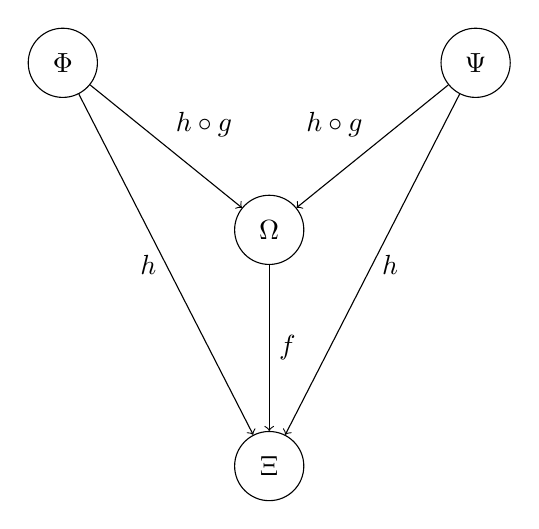
\begin{tikzpicture}[->,node distance=3cm]
\node[state] (Xi)                                        {$\Xi$}   ;
\node[state] (Omega) [above of=Xi]                       {$\Omega$};
\node[state] (Phi)   [above left of=Omega,  xshift=-5mm] {$\Phi$}  ;
\node[state] (Psi)   [above right of=Omega, xshift=5mm]  {$\Psi$}  ;
\path (Phi)   edge node [left]        {$h$}         (Xi)
              edge node [above right] {$h \circ g$} (Omega)
      (Psi)   edge node [right]       {$h$}         (Xi)
              edge node [above left]  {$h \circ g$} (Omega)
      (Omega) edge node [right]       {$f$}         (Xi);
\end{tikzpicture}
\end{center}

\begin{defin}
A formula $\Delta$ is a \textbf{canonical intersection} of two formulae $\Phi$ and $\Psi$, if and only if 
$\Delta$ is equivalent to $\Phi\cap\Psi$ and every function that assigns $\Phi$ and $\Psi$ to the same formula also assigns $\Delta$ to that formula.
We will introduce the following notation to express this:
\begin{align*}
\dfrac{\Phi \cap \Psi}{\Delta} \iff (\Phi\cap\Psi\equiv\Delta\land(\forall h : (\Phi\lhd h =\Psi\lhd h) \implies \Delta\lhd h=\Phi\lhd h))
\end{align*}
\end{defin}

\begin{lem}
If $\Delta$ is the canonical intersection of $\Phi$ and $\Psi$ then every free variable that appears in $\Delta$ must also appear in $\Phi$ and $\Psi$.
\begin{align*}
\dfrac{\Phi\cap\Psi}{\Delta}\implies\Delta^\mathbb{V}\subseteq\Phi^\mathbb{V}\cup\Psi^\mathbb{V}
\end{align*}
\end{lem}
\begin{proof}
Let us assume the negation.
Namely that there exists some free variable in $\Delta$ that is not in $\Phi$ or $\Psi$
\begin{align*}
\exists x : x \in \Delta^\mathbb{V} \land \neg (x \in \Phi^\mathbb{V}) \land \neg (x \in \Psi^\mathbb{V})
\end{align*}
Let us consider some function $h$ such that $\Phi\lhd h=\Psi\lhd h$.
By the definition of canonical intersection we know that it must be the case that $\Delta\lhd f = \Phi\lhd f$.
Now it must be the case that $h$ maps $x$ to some value, so we will make a new function $h'$ such that
for all values other than $x$, $h'$ behaves the same way as $h$, but for $h'(x)$ it maps to anything other than $h(x)$.
It doesn't matter what as long as it is different from what $h$ maps $x$ to.
Now it is clear that because $h'$ is the same as $h$ on the domains of $\Phi$ and $\Psi$, that $\Phi\lhd h' = \Phi\lhd h = \Psi\lhd h = \Psi\lhd h'$.
From our definition we can conclude that $\Delta \lhd h' = \Delta \lhd h$, thus via our first lemma $h' \mid \Delta^\mathbb{V} = h \mid \Delta^\mathbb{V}$.
However we already know this is false because we asserted that $h'(x) \neq h(x)$.
From this contradiction we can conclude that no such $x$ can exist.

\end{proof}

\begin{defin}
\textbf{The arrow number} of a formula $\Phi$, denoted $\Phi^\rightarrow$, will be defined as follows:
\begin{align*}
(\Phi_1\rightarrow\Phi_2)^\rightarrow &= 1 + \Phi_1^\rightarrow + \Phi_2^\rightarrow \\
(\neg\Phi_0)^\rightarrow &= \Phi_0^\rightarrow \\
\Phi \in \mathbb{V} \implies \Phi^\rightarrow &= 0\\
\Phi \in \mathbb{A} \implies \Phi^\rightarrow &= 0
\end{align*}
\end{defin}

This can also be thought of as the number of arrows appearing in the string that represents our formula.

\begin{thm}
Either the intersection of two formula is empty or there is a canonical intersection.
\begin{align*}
\forall \Phi,\Psi \in \mathcal{F} : \left(\Phi \cap \Psi = \left\{\right\} \lor \exists \Omega : \dfrac{\Phi \cap \Psi}{\Omega} \right)
\end{align*}
\end{thm}
\begin{proof}
This proof will be performed via structural induction.
To start we verify that this is in fact the case for atoms.
$\Phi \cap \Psi$ is the empty set if the atoms are different and is $\Phi$ if the atoms are the same.
This is pretty clear because no assignment can change a formula consisting only of an atom.
If $\Phi$ is the intersection it must be canonical because all assignments of $\Phi$ are also $\Phi$.

We can also see that for two free variables there is always a canonical intersection.
All the functions that assign two free variables to the same well formed formula are functions such that $f(\Phi) = f(\Psi)$ thus if we choose
our canonical intersection to be either $\Phi$ or $\Psi$ we will that this is indeed a intersection and it must be canonical.

Let us now consider that one of our statements is a free variable but the other is not.
Let's say that 

Next we can see that if $\Phi \cap \Psi \equiv \Omega$
\begin{align*}
\neg \Phi \cap \neg \Psi \equiv \neg \Omega
\end{align*}
but if $\Phi \cap \Psi = \{\}$ then
\begin{align*}
\neg \Phi \cap \neg \Psi = \{\}
\end{align*}
this means that negation upholds our property.

We now have an inductive proof that our proposition holds for all statements with arrow number $0$.

Now we will consider statements that do not have arrow number $0$.
We have already shown that statements with a negation at the top level are equivalent to a formula or empty set if removing the negation leaves us with formulae that have such an intersection, so we may go ahead and just consider statements that have an implication at the top level.
We consider
\begin{align*}
(\Phi_1 \rightarrow \Phi_2) \cap (\Psi_1 \rightarrow \Psi_2)
\end{align*}
Now if either $\Phi_1 \cap \Psi_1 = \{\}$ or $\Phi_2 \cap \Psi_2 = \{\}$ it is clear that the composite statement must be empty.
So we will only consider the case where $\exists \Lambda_1 : \Phi_1 \cap \Psi_1 \equiv \Lambda_1$ and $\exists \Lambda_2 : \Phi_2 \cap \Psi_2 \equiv \Lambda_2$.

Since $\Phi_1\cap \Psi_1 \equiv \Lambda_1$ we know, by lemma 3, that there is an assignment function $f$ that assigns both $\Phi_1$ and $\Psi_1$ to $\Lambda_1$.
Let us consider an arbitrary member of the intersection of $(\Phi_1\rightarrow\Phi_2)$ and $(\Psi_1\rightarrow\Psi_2)$, let us call it $(\Xi_1\rightarrow\Xi_2)$.
If we call the function that assigns both $(\Phi_1\rightarrow\Phi_2)$ and $(\Psi_1\rightarrow\Psi_2)$ to $(\Xi_1\rightarrow\Xi_2)$, $h$.
$h$ must assign $\Phi_1$ and $\Psi_1$ to the same well formed formula (namely $\Xi_1$),
thus by the definitions of equivalent formulae it must be the case that there is a function $g$ that assigns $\Lambda_1$ to $\Phi_1\lhd h$ and $\Psi_1\lhd h$.
Thus
\begin{align*}
\Phi \lhd (f\diamond g) = \Phi_1 \lhd h \\
\Psi \lhd (f\diamond g) = \Psi_1 \lhd h
\end{align*}
From Lemma 1 we then show that
\begin{align*}
(f\diamond g) \mid \Phi_1^\mathbb{V} \cup \Psi_1^\mathbb{V} = h \mid \Phi_1^\mathbb{V} \cup \Psi_1^\mathbb{V} 
\end{align*}
Now it is trivially true that if $\mathrm{id}$ is the function that maps every free variable to itself.
\begin{align*}
(\mathrm{id}\diamond h) = h
\end{align*}
So if we define two new functions $f'$ and $g'$ such that
\begin{align*}
f' (x) = \begin{cases}
f (x) & x \in \Phi_1^\mathbb{V} \cup \Psi_1^\mathbb{V} \\ 
x & \mathrm{otherwise}
\end{cases}\\
g'(x) = \begin{cases}
g (x) & x \in \Phi_1^\mathbb{V} \cup \Psi_1^\mathbb{V} \\ 
h (x) & \mathrm{otherwise}
\end{cases}
\end{align*}
It then must be the case that
\begin{align*}
(f'\diamond g') = h
\end{align*}
This means that for any formula $\Xi$ in the intersection, that
\begin{align*}
((\Phi_1\rightarrow\Phi_2)\lhd f')\lhd g' = \Xi \\
((\Psi_1\rightarrow\Psi_2)\lhd f')\lhd g' = \Xi
\end{align*}
And since $f'$ is not dependent on $\Xi$ we can say that
\begin{align*}
(\Phi_1\rightarrow\Phi_2)\cap(\Psi_1\rightarrow\Psi_2)
&= ((\Phi_1\rightarrow\Phi_2)\lhd f')\cap((\Psi_1\rightarrow\Psi_2)\lhd f') \\
&= (\Lambda_1\rightarrow(\Phi_2\lhd f'))\cap(\Lambda_1\rightarrow(\Psi_2\lhd f'))
\end{align*}
Since $\Lambda_1$ is already equal to itself, any assignment of $\Lambda_1$ will be equal to itself.
Thus an assignment will assign both $(\Phi_2\lhd f')$ and $(\Psi_2\lhd f')$ to the same formula if and only if it assigns both $(\Lambda_1\rightarrow(\Phi_2\lhd f'))$ and $(\Lambda_1\rightarrow(\Psi_2\lhd f'))$ to the same formula.
\begin{equation*}
(\Phi_2\lhd f')\lhd k =(\Psi_2\lhd f')\lhd k \iff
(\Lambda_1\rightarrow(\Phi_2\lhd f')) \lhd k = (\Lambda_1\rightarrow(\Psi_2\lhd f')) \lhd k
\end{equation*}
From this fact it is clear that $(\Phi_2\lhd f')\cap(\Psi_2\lhd f')$ is empty if and only if $(\Lambda_1\rightarrow(\Phi_2\lhd f'))\cap(\Lambda_1\rightarrow(\Psi_2\lhd f'))$ is also empty.
If $(\Phi_2\lhd f')\cap(\Psi_2\lhd f')$ is non-empty we see that
\begin{align*}
\forall k :
(\Phi_2\lhd f') \lhd k = (\Psi_2\lhd f') \lhd k
&\iff ((\Lambda_1\lhd k)\rightarrow ((\Phi_2\lhd f')\lhd k)) = ((\Lambda_1\lhd k)\rightarrow ((\Psi_2\lhd f')\lhd k)) \\
&\iff (\Lambda_1\rightarrow (\Phi_2\lhd f'))\lhd k = (\Lambda_1\rightarrow (\Psi_2\lhd f'))\lhd k
\end{align*}
Thus from here if $(\Phi_2\lhd f')\cap(\Psi_2\lhd f') \equiv \Omega$ then by lemma 3 there must be an assignment $k$ from both $(\Phi_2\lhd f')$ and $(\Psi_2\lhd f')$ to $\Omega$, 
which entails that every assignment into the intersection must be of the form $(k \diamond l)$.
From the above result this means that every assignment from $(\Lambda_1\rightarrow (\Phi_2\lhd f'))$ and $(\Lambda_1\rightarrow (\Psi_2\lhd f'))$ into their intersection must also be of the form $(k \diamond l)$.
If we take $(\Lambda_1\rightarrow (\Psi_2\lhd f'))\lhd k$, it must be a formula and it must be equivalent to the intersection.
Thus if there is some formula that is equivalent to $(\Phi_2\lhd f')\cap(\Psi_2\lhd f')$ there must also be an formula that is equivalent to $(\Phi_1 \rightarrow \Phi_2) \cap (\Psi_1\rightarrow \Psi_2)$.

Now we will take a moment to prove that $|(\Phi_2\lhd f')^\mathbb{V}\cup(\Psi_2\lhd f')^\mathbb{V}| \leq |(\Phi_1\rightarrow\Phi_2)^\mathbb{V} \cup (\Psi_1\rightarrow\Psi_2)^\mathbb{V}|$.
\begin{subproof}
We can use lemma 3 to show
\begin{align*}
(\Phi_2\lhd f')^\mathbb{V}\cup(\Psi_2\lhd f')^\mathbb{V}
= \bigcup_{\delta \in \Phi_2^\mathbb{V}\cup\Psi_2^\mathbb{V}}(f'(\delta))^\mathbb{V}
\end{align*}
And by definition we can also say that:
\begin{align*}
(\Phi_1\rightarrow\Phi_2)^\mathbb{V} \cup (\Psi_1\rightarrow\Psi_2)^\mathbb{V} =
\Phi_1^\mathbb{V}\cup\Phi_2^\mathbb{V} \cup \Psi_1^\mathbb{V}\cup\Psi_2^\mathbb{V}
\end{align*}

\end{subproof}

\end{proof}

\begin{thm}
There is no proof of $A \rightarrow A$ in the \L ukasiewicz system that is less than 5 steps long.
\end{thm}
\begin{proof}
In order to prove that no such proof exists we will attempt to construct such a proof.
We will despite our best efforts fail to do so demonstrating the impossibility of the task.

We will start our proof at the end.
We know that the statement $A \rightarrow A$ must appear in the proof,
and that any steps after it are extraneous and can be removed.
Thus $A \rightarrow A$ must be the last step of the proof.
We will label this step $\alpha$

\begin{align*}
A \rightarrow A \tag*{($\alpha$)}\\
\end{align*}

We also know that $A \rightarrow A$ does not fit the form of any of our axioms.
This means that we must have arrived at it from modus ponens.

\begin{align*}
A \rightarrow A \tag*{Modus Ponens ($\alpha$)}\\
\end{align*}

Since we arrived at this from modus ponens we know that there must be earlier statements of the form $\phi$ and $\phi \rightarrow (A \rightarrow A)$.
Since all statements are finite we also know that there is no $\phi$ such that

\begin{align*}
\phi = \phi \rightarrow (A \rightarrow A)
\end{align*}

Thus the two statements must be separate.

\begin{gather*}
\phi \tag{$\gamma$}\\
\phi \rightarrow (A \rightarrow A) \tag{$\beta$}\\
A \rightarrow A \tag*{Modus Ponens ($\alpha$)}\\
\end{gather*}

We can express $\phi \rightarrow (A \rightarrow A)$ as a statement of L.S.1 if $\phi = A$,
however doing so would mean that our proof would need to include a proof of $A$.
Since $A$ clearly is independent of our axioms we know that the statement cannot be a reference to L.S.1.

If we try to write the same statement as L.S.2 we will find it impossible.

\begin{gather*}
\phi \rightarrow (A \rightarrow A) = (\psi \rightarrow (\chi \rightarrow \omega)) \rightarrow ((\psi \rightarrow \chi) \rightarrow (\psi \rightarrow \omega)) \\
\phi = (\psi \rightarrow (\chi \rightarrow \omega)), A \rightarrow A = (\psi \rightarrow \chi) \rightarrow (\psi \rightarrow \omega) \\
\phi = (\psi \rightarrow (\chi \rightarrow \omega)), A = \psi \rightarrow \chi, A = \psi \rightarrow \omega \\
\end{gather*}

Since $A$ cannot be of the form $\psi \rightarrow \chi$ (nor the form $\psi \rightarrow \omega$) there is no instantiation of L.S.2 of the form $\phi \rightarrow (A \rightarrow A)$.

If we set $\phi$ equal to $\neg A \rightarrow \neg A$ we will find that L.S.3 allows us to conclude our statement.

\begin{gather*}
\neg A \rightarrow \neg A \tag{$\gamma$}\\
(\neg A \rightarrow \neg A) \rightarrow (A \rightarrow A) \tag*{L.S.3 ($\beta$)} \\
A \rightarrow A \tag*{Modus Ponens ($\alpha$)}\\
\end{gather*}

Now using the same thought process as $A \rightarrow A$ we can show that $\neg A \rightarrow \neg A$ must be derived via modus ponens.
This gives us a proof of the form:

\begin{gather*}
\psi \tag{$\eta$}\\
\psi \rightarrow (\neg A \rightarrow \neg A) \tag{$\delta$} \\
(\neg A \rightarrow \neg A) \rightarrow (A \rightarrow A) \tag*{L.S.3 ($\beta$)} \\
\neg A \rightarrow \neg A \tag*{Modus Ponens ($\gamma$)}\\
A \rightarrow A \tag*{Modus Ponens ($\alpha$)}\\
\end{gather*}

Now since we are looking for a proof with 4 steps we know that it must be the case that $\psi$ is equal to $(\neg A \rightarrow \neg A) \rightarrow (A \rightarrow A)$, otherwise we would have 5 steps.

\begin{gather*}
((\neg A \rightarrow \neg A) \rightarrow (A \rightarrow A)) \rightarrow (\neg A \rightarrow \neg A) \\
(\neg A \rightarrow \neg A) \rightarrow (A \rightarrow A) \tag*{L.S.3} \\
\neg A \rightarrow \neg A \tag*{Modus Ponens}\\
A \rightarrow A \tag*{Modus Ponens}\\
\end{gather*}

Now we need to check whether the first statement can be a instantiation of one of our axioms.
If we check we find that there are no values of $\phi$, $\psi$ and $\chi$ for which the our statement is an instantiation of any of the axioms.

Now we backtrace to the last descision we made.
We chose to represent $\phi \rightarrow (A \rightarrow A)$ as L.S.3.
Since that arrived us at an incorrect conclusion we know that it cannot be the case that in a four step proof that step is introduced by L.S.3.
Since we have removed all of the axioms as possibilites to introduce $\phi \rightarrow (A \rightarrow A)$  we know that it is introduced by modus ponens.

\begin{gather*}
\phi \\
\psi \\
\psi \rightarrow (\phi \rightarrow (A \rightarrow A)) \\
\phi \rightarrow (A \rightarrow A) \tag*{Modus Ponenes} \\
A \rightarrow A \tag*{Modus Ponens}\\
\end{gather*}

Since we have 5 claims here we know that in order to reduce our proof to 4 steps we must have two of them that are equal.
It is clear that no statement containing $\phi$ can be equal to $\phi$ and the same goes for $\psi$.
We also know that if a statement $\chi$ that relies on a statement $\omega$, it must be the case that $\chi \neq \omega$ otherwise our proof would be circular.

Of the remaining statments that could be equal there is only one pair that has the same form.
This leaves us to say that $\phi = \psi$. 

\begin{gather*}
\phi \\
\phi \rightarrow (\phi \rightarrow (A \rightarrow A)) \\
\phi \rightarrow (A \rightarrow A) \tag*{Modus Ponenes} \\
A \rightarrow A \tag*{Modus Ponens}\\
\end{gather*}

Our remaining statements must be instantiations of our axioms because any use of modus ponens would add new steps to the proof.
If we start with the sentence $\phi \rightarrow (\phi \rightarrow (A \rightarrow A))$ we will find it can only be instantiated by L.S.1.

\begin{gather*}
A \rightarrow A \\
(A \rightarrow A) \rightarrow ((A \rightarrow A) \rightarrow (A \rightarrow A)) \tag*{L.S.1} \\
(A \rightarrow A) \rightarrow (A \rightarrow A) \tag*{Modus Ponenes} \\
A \rightarrow A \tag*{Modus Ponens}\\
\end{gather*}

Now in order to make this proof valid we must proof $A \rightarrow A$ in 1 step.
This would require the instantiation of an axiom and we already know that this is impossible.

Thus there is no proof of $A \rightarrow A$ that is 4 steps or shorter.
\end{proof}

We can note that the methodology for determining the shortest possible proof is to work backwards from the desired conclusion. We can begin to formalize this into a general approach by observing which axioms are utilized in our proof. Note that Modus Ponens was applied to obtain the final statement and L.S.1 was applied to our initial statement to create a second:

\begin{gather*}
	\phi \tag*{Given (X)} \\
	\phi \rightarrow (\Xi \rightarrow \phi) \tag*{L.P.1 on X (X+1)} \\
\end{gather*}

and 

\begin{gather*}
	\Sigma \rightarrow \psi \tag*{Some axiom (Y-1)} \\
	\psi \tag*{MP on Y-1 (Y)} \\
\end{gather*}

where we seek to prove that $\phi \rightarrow \psi$. We can account for $4$ of the necessary $5$ steps we've proven that we need to create a valid argument. The fifth step linking the our two pairs must utilize one of our axioms, meaning that we have three options: \\

L.S.1
\begin{gather*}
	(\phi \rightarrow (\Xi \rightarrow \phi)) \rightarrow ((\Sigma \rightarrow \psi) \rightarrow (\phi \rightarrow (\Xi \rightarrow \phi))
\end{gather*} \\

L.S.2
\begin{gather*}
	(\phi \rightarrow (\Xi \rightarrow \phi)) \rightarrow ((\phi \rightarrow \chi) \rightarrow (\phi \rightarrow \phi))
\end{gather*} \\

L.S.3
\begin{gather*}
(\neg\neg \phi \rightarrow \neg\neg(\Sigma \rightarrow \phi)) \rightarrow (\neg(\Sigma \rightarrow \psi) \rightarrow \neg\phi)
\end{gather*} \\

L.S.3 doesn't directly apply to our given pairs; it was only included due to the technical equivalence of $(\phi \rightarrow (\Sigma \rightarrow \phi)$ to $(\neg \neg \phi \rightarrow \neg\neg(\Sigma \rightarrow \phi))$ (by virtue of the definition of $\neg$). As such, we'll disregard it and only move forward with L.S.1 and L.S.2. \\



\end{document}
